% arara: pdflatex: { synctex: yes }
% arara: makeindex: { style: ctuthesis }
% arara: bibtex

% The class takes all the key=value arguments that \ctusetup does,
% and a couple more: draft and oneside
\documentclass[twoside]{template/ctuthesis}

\ctusetup{
	preprint = \ctuverlog,
%	mainlanguage = english,
%	titlelanguage = czech,
	mainlanguage = czech,
	otherlanguages = {english},
	title-czech = {Bakalářský projekt},
	title-english = {Bachelor's Project},
	subtitle-czech = {Baseline k bakalářské práci},
	subtitle-english = {Baseline to Bachelor's Project},
	doctype = B,
	faculty = F3,
	department-czech = {Katedra měření},
	department-english = {Department of Measurment},
	author = {Ladislav Štefka},
	supervisor = {doc. Ing. Radislav Šmíd, Ph.D},
	supervisor-address = {Ústav X, \\ Uliční 5, \\ Praha 99},
	supervisor-specialist = {...},
	fieldofstudy-english = {Cybernetics and Robotics},
	fieldofstudy-czech = {Kybernetika a Robotika},
	keywords-czech = {LoRa, IoT},
	keywords-english = {LoRa, IoT},
	day = 2,
	month = 2,
	year = 2018,
	specification-file = {ctutest-zadani.pdf},
}

\ctuprocess

\addto\ctucaptionsczech{%
	\def\supervisorname{Vedoucí}%
	\def\subfieldofstudyname{Studijní program}%
}

\ctutemplateset{maketitle twocolumn default}{
	\begin{twocolumnfrontmatterpage}
		\ctutemplate{twocolumn.thanks}
		\ctutemplate{twocolumn.declaration}
		\ctutemplate{twocolumn.abstract.in.titlelanguage}
		\ctutemplate{twocolumn.abstract.in.secondlanguage}
		\ctutemplate{twocolumn.tableofcontents}
		\ctutemplate{twocolumn.listoffigures}
	\end{twocolumnfrontmatterpage}
}

% Theorem declarations, this is the reasonable default, anybody can do what they wish.
% If you prefer theorems in italics rather than slanted, use \theoremstyle{plainit}
\theoremstyle{plain}
\newtheorem{theorem}{Theorem}[chapter]
\newtheorem{corollary}[theorem]{Corollary}
\newtheorem{lemma}[theorem]{Lemma}
\newtheorem{proposition}[theorem]{Proposition}

\theoremstyle{definition}
\newtheorem{definition}[theorem]{Definition}
\newtheorem{example}[theorem]{Example}
\newtheorem{conjecture}[theorem]{Conjecture}

\theoremstyle{note}
\newtheorem*{remark*}{Remark}
\newtheorem{remark}[theorem]{Remark}

\setlength{\parskip}{5ex plus 0.2ex minus 0.2ex}

% Abstract in Czech
\begin{abstract-czech}
\end{abstract-czech}

% Abstract in English
\begin{abstract-english}
\end{abstract-english}

% Acknowledgements / Podekovani
\begin{thanks}

\end{thanks}

% Declaration / Prohlaseni
\begin{declaration}
\end{declaration}

% Only for testing purposes
\listfiles
\usepackage[pagewise]{lineno}
\usepackage{lipsum,blindtext}
\usepackage{mathrsfs} % provides \mathscr used in the ridiculous examples
\usepackage{hyperref}
\usepackage{siunitx}
\usepackage{caption}
\usepackage{subcaption}

\newcommand{\todo}[1]{\textcolor{red}{\textbf{TODO: #1}}\PackageWarning{TODO:}{#1!}}

\newcommand{\question}[1]{\textcolor{blue}{\textbf{QUESTION: #1}}\PackageWarning{QUESTION:}{#1!}}

\newcommand{\answer}[1]{\textcolor{magenta}{\textbf{ANSWER: #1}}\PackageWarning{ANSWER:}{#1!}}

\begin{document}

\maketitle

%!TEX ROOT=ctutest.tex
\chapter{Úvod}

    Funkčnost a spolehlivost technických zařízení se výrazně podepisuje na provozních nákladech a bezpečnosti moderních systémů v průmyslu po celou dobu jejich fungování. 
    Za pomoci diagnostiky stavu zařízení a následné údržby je cílem každé firmy minimalizovat ztráty a rozsah škod způsobených jejich poruchami nebo úplným selháním. Tato diagnostika stavu a údržba zařízení je prováděna  všude kolem nás, ve všech technologických oblastech, od těžkých strojních přístrojů (přístavní jeřáby, důlní zařízení), po leteckou techniku (letadla, helikoptéry) až po jemná biotechnologická zařízení, jako jsou např. kardiostimulátory.
    Na otázku, jak efektivně vyřešit poruchy nejrůznějších strojů, existuje jednoduchá odpověď - předejít jejím vznikům. Tato myšlenka nese filosofii konceptů Condition Based Maintenence (CBM) a Predictive Maintenence, které jsou jedním ze základních stavebních kamenů moderní diagnostiky zařízení v průmyslu.
    
    Preventivní predeterminovaná údržba s pravidelnými kontroly a diagnostikou stavu zařízení byla po dlouhou dobu v minulosti nejspolehlivější metodou, jak předejít poruše stroje. V dnešní době, kdy je ale kladen důraz na maximální efektivnost, nese tento koncept údržby mnohá úskalí. Pravidelné kontroly zvyšují finanční náklady na provoz, mrhají jak lidskými tak materiálními zdroji, často musí kvůli nim být pozastavena výroba a i přes to neeliminují riziko poruchy.
    
    Prediktivní údržba podle technického stavu (CBM) díky moderním technologiím dnešní doby, které umožňují monitorovat a diagnostikovat stav zařízení v reálném čase, dokáže předvídat poruchu ještě před tím, než k ní dojde, a rozhoduje tak o provedení údržby v tu chvíli, kdy ji je opravdu třeba. Tento koncept je tedy proto v mnoha aplikacích výhodnější, přináší časové, pracovní a materiálové úspory a je velice vhodný zejména pro zařízení, jejichž selhání má fatální následky.

\subsection{Diagnostika stavu rotačních zařízení}
    K selhání motorů může dojít mnoha způsoby, ačkoliv fakta ukazují, že 40 až 90 \% poruch je zapříčiněno defektem ložisek. Tyto poruchy navíc často způsobují selhání celého motoru, a proto se jejich diagnostika a  sledování stavu stává důležitým úkolem. 
    Pro monitorování stavu ložisek se nejčastěji používá vibrační analýza a měření teploty. Tyto veličiny reflektují stav ložisek, jejich mechanické namáhání, opotřebení materiálů, vznikající trhliny a tvarové nedokonalosti.
    Z vlastností vibračního signálu lze identifikovat příznaky přicházející poruchy ložisek, avšak tento úkol není vůbec snadný. Pro přesnou expertízu je třeba vědět, které charakteristiky vibračního signálu je třeba sledovat a jakým způsobem jsou spojeny s vlastnostmi ložiska.     
    

\subsection{Monitorování zařízení v rámci IIoT}
    V dnešních dnech je fenomén Internet of Things (IoT) česky Internet věcí jedním z nejcitovanějších témat v technologicky zaměřených médiích. Pro mnohé se ale tento pojem stal symbolem své pouze jedné větve - spotřebitelského internetu věcí, který je z popularizačního hlediska zajímavější, zaměřen na chytrá města a domácnosti.\\
    Mnohem větší význam, ale nese Industrial Internet of Things (IIoT) česky Průmyslový internet věcí, často označovaný jako Průmysl 4.0. IIoT v první řadě poskytuje lepší přehled o aktivitách v průmyslové výrobě a to prostřednictvím monitorujících senzorů, konektivity a cloud computingu.
    Díky zpětné vazbě získané z datové analýzy umožňuje transformovat a především optimalizovat výrobní operace, což zvyšuje zejména produktivitu, efektivnost a náklady.\\
    IIoT je tedy klíčovým faktorem umožňující realizovat prediktivní údržbu a CBM.\\
    
    

\subsection{LPWAN a vibrační analýza}
    
    Bezdrátový IIoT představuje další větev Průmyslového Internetu věcí. Jeho využití, ale přináší řadu úskalí jako je dovolená šířka pásma, elektromagnetická kompatibilita (EMC), spolehlivost komunikace a výdrž na baterii, která se výrazně snižuje díky použití bezdrátových přijímačů a vysílačů. Obecně lze říci, že díky těmto důvodům je pro průmyslové aplikace vždy vhodnější využití drátové komunikace nežli bezdrátové. 
    Většina stávajících řešení poskytujících vibrační analýzu využívá proto pro komunikaci ve výrobních halách již dobře dostupná rozhraní jako Ethernet Powerlink nebo HART (Highway Addressable Remote Transducer Protocol).\\
    V mnoha případech je ale použití drátových technologií problematické. Často jsou také opomíjena rotační zařízení například v elektrárnách, tunelech nebo na rozlehlých stavebních plochách, kde by vytvoření drátové sítě bylo velmi nákladné, či úplně nemožné a jejichž monitorování by tak nebylo možné. V těchto případech je tedy nasnadě využití bezdrátových komunikačních sítí LPWAN (Low Power Wide Area Network) jako například LoRa, SigFox či NB-IoT. Tyto sítě se vyznačují hvězdicovitou architekturou, kdy koncová zařízení odesílají data do bran, které jsou připojena k internetu na cloudovou platformu.  

\subsection{Cíl práce}
    
    Cílem této práce bylo navrhnout a realizovat komplexní pokročilý systém pro monitorování stavu průmyslových zařízení pomocí pokročilé analýzy vibrací a teploty.\\
    Sytém se bude odlišovat od existujících zařízení na trhu zejména svoji konfigurovatelností. Uživatel bude moci pohodlně ve webovém prostředí měnit parametry monitorovací jednotky, díky čemuž bude moci přizpůsobit zpracování monitorovaných veličin a dosáhnout tak různorodějších a pokročilejších analýz.\\
    
    Důraz bude kladen zejména na cenu, dostupnost a univerzální použití. Jako komunikační médium se bude využívat LPWAN síť LoRa s velkým dosahem, ale nízkým datovým tokem, což se může na první pohled zdát jako nesmyslný krok. Tato technologie ale umožní sledovat stav rotačních zařízení nejen v chytrých průmyslových výrobnách ale i na rozsáhlých plochách pro velké vzdálenosti, což odliší systém od existujících řešení a umožní jej používat i v prostředích, kde nasazení podobného systému bylo komplikované jako například větrné elektrárny, tunely nebo rozlehlé stavební plochy.\\
    
    Mimo jiné bude pozornost věnována flexibilitě celého systému prostřednictvím použití databázového modelu a RESTového serveru, které umožní poskytnutí naměřených dat aplikacím třetích stran, které zákazníci budou moci zpracovávat podle svých požadavků ve vlastních systémech.
    
Zdroje

https://www.bozpinfo.cz/josra/prediktivni-udrzba-metody-technicke-prognostiky-seznameni-se-s-problematikou

Industry 4.0: The Industrial Internet of Things

\question{TYPOGRAFIE: prvni odstavec}


\part{Praktická část}

%!TEX ROOT=ctutest.tex

\chapter{Komunikační řetězec – IoT aplikace}
\question{Popis komunikačního řetězce v teoretickém úvodu?}
\answer{V BP může být v teor. části obecnější popis = bez konkrétních součástek, nastavení apod., v části Realizace pak navázat popisem konkrétní implementace - součástky, nastavení, atd. }


\section{LoRa Node}
    LoRa Node je koncové zařízení, které komunikuje se senzory, zpracovává naměřená data a odesílá je v podobě LoRa paketů do LoRa brány.

\subsection{Výběr komponent}

\subsubsection{Mikrokontrolér (MCU) – STM32L0RZ73 }

    Výběr výpočetní jednotky byl ovlivněn zejména dvěma požadavky – dostatečným výpočetním výkonem, který je třeba pro zpracování signálu z akcelerometru, a nízkou spotřebou. Tyto požadavky jdou ovšem zcela proti sobě, a nakonec byl tak jako kompromis použit procesor z „low power“ série mikrokontrolérů od firmy STM – STM32L0RZ73. 
    
    \question{Doplnit o specifikaci MCU??}
    
\answer{Ano, v BP udělat přehled relevantních parametrů a architektury}

\subsubsection{LoRa modul – I-NUCLEO-SX1272D}
    $\text{LoRa}^{\text{TM}}$ je uzavřená technologie, kterou licencuje a vyvíjí firma SemTech. Všechny čipy podporující tuto modulaci nesou označení SX127x. Na trhu se nachází nepřeberné množství LoRa modulů, které se liší především výstupním výkonem, komunikačním rozhraním a cenou.
    
    Protože jsem chtěl vytvořit vlastní LoRa bránu a nevyužívat oficiální brány, bylo třeba použít pouze LoRa modul a nikoliv LoRaWAN modul, který má v sobě implementovaný LoRaWAN protokol a slouží právě pro komunikaci s oficiálními branami. K tomuto účlu posloužil LoRa modul s čipem SX1272 přímo od společnosti ST, který byl součástí vývojářského kitu, který jsem dostal a který lze zapojit přímo do Nuclea.
    
    
    \href{https://www.st.com/en/evaluation-tools/i-nucleo-sx1272d.html}{Source}




\subsubsection{Teplotní senzor – TMP75}

    TMP75 je digitální teplotní čidlo od firmy Texas Instruments, které pro měření využívá 12bitový převodník. Jedná se o poměrně rozšířený senzor komunikující po I2C sběrnici, který je díky své malé spotřebě vhodný zejména do zařízení, které jsou poháněny baterií.
    
    \question{Doplnit o specifikaci senzorů??}

\subsubsection{Senzor vibrací – ADXL1001}

    \todo{!!!Podle čeho vybrat akcelerometr do naší aplikace???}
    
    \answer{rozsah, noise floor u analogového/ rozlišení u digitálního, šířka pásma/vzorkovací frekvence}




\subsection{Návrh zapojení}

    Zapojení LoRa Node je vyřešeno za pomocí vývojářského kitu NUCLEO a nepájivého pole, do kterého jsou připojeny senzory. Jedná se zatím pouze o první verzi pro testovací účely. Oba dva senzory jsou napájeny z Nuclea a fungují na 3.3 V logice. K senzorům jsou přidány kondenzátory pro blokování napájení. Výsledné zapojení lze vidět na obrázku...
    
    \todo{!!!Doplnit Schéma zapojení}
    
    \todo{!!!Doplnit foto}


\subsection{Softwarové nástroje}

    Softwarový vývoj postavený na platformě ST může probíhat několika odlišnými způsoby. Lze využívat knihovnu obsahující pouze registry procesoru – CMSIS, nízkoúrovňovou knihovnu LL (Low Level) nebo již komplexní knihovny HAL (Hardware Abstraction Layer). V této práci byla použita kombinace všech tří přístupů. Obsluha komunikace MCU přes UART byla například naprogramována pouze pomocí CMSIS, obsluha AD převodníku pomocí LL a obsluha I2C pomocí HAL.
    
    \question{Mělo by to byt všechno unifikované???}
    
    \answer{Nemusí být, pokud je to zdůvodnitelné - např. někde něco chybí}

\subsection{Funkčnost LoRa Node}

    Průběh programu je následující. Po restartování MCU dojde k inicializaci periferií a příslušné nastavení GPIO pinů. V dalším kroku dochází ke čtení hodnot ze senzorů, jejich naformátování a vytvoření zprávy, která je odeslána prostřednictvím LoRa modulu. 
    Po odeslání paketu přechází zařízení do SLEEP módu, ze kterého je po 30 sekundách pomocí RTC obvodu probuzeno a dochází opět k dalšímu čtení dat ze senzorů a odeslání zprávy.

\subsection{Způsob komunikace – formát odeslaných dat}

    \todo{!!!Vymyslet přesně daný formát zprávy}




\section{LoRa brána}

    \todo{Otestovat dosah brány}
    
    \todo{Změřit spotřebu a propustnost}
    

    Brána (Gateway) slouží jako prostředník mezi jednotlivými koncovými zařízeními (LoRa Nodes) a cloudovou službou. Její hlavní funkcí je tedy příjem LoRa paketů a jejich přeposílání přes IP protokol do cloudu.

\subsection{Výběr komponent}
    
    \subsubsection{Mikrokontrolér – Raspberry Pi}
        Vlastní LoRa brána může být postavena spíše minimalisticky za použití určitého mikrokontroléru, tedy se slabým výkonem, ale nízkou cenou a spotřebou – například jako další STM32 jednotka s ethernet nebo WiFi modulem nebo pomocí oblíbeného vývojářského čipu ESP8266/ESP32. 
        Opačný přístup by bylo postavení brány s výpočetně silnějším počítačem a operačním systémem, tedy s velkým výkonem, ale vyšší cenou a spotřebou.

        Pro realizaci brány bylo nakonec použité \textbf{Raspberry Pi}, konkrétně verze 3 model B s operačním systémem Raspbian. 
        Motivací výběru Raspberry po zvážení kritérií popsaných výše byl zejména dostatečný výpočetní výkon, vývojářská podpora a výhody operačního systému. Spotřeba brány není tak důležité kritérium jako u koncových zařízení, protože brána může mít stálý zdroj napájení. Raspberry byl tedy jakýsi kompromis mezi výkonem a cennou. Další plus, které toto řešení nabízí je veliká univerzálnost – na RPi lze naprogramovat mnoho aplikací, které by přizpůsobily chování celého systému podle konkrétních požadavků zákazníka (například lokální záloha dat z LoRa Nodes, pouze lokální řešení bez cloudové služby \ldots).
        
        \question{Doplnit o technické parametry Raspberry?}
        
        \answer{pouze ty podstatné}
        
    \subsubsection{LoRa modul – I-NUCLEO-SX1272D}

        Pro komunikaci s koncovými zařízeními byl využit stejný LoRa modul jako pro koncová zařízení – \textbf{I-NUCLEO-SX1272D}.

        Bohužel tento modul je určený pro vývojovou desku Nucleo, čemuž odpovídá i jiná DPS, a proto bylo třeba propojit GPIO piny Raspberry a modulu drátky. V další verzi by bylo určitě vhodné vytvořit desku s LoRa modulem, která by přímo seděla na rozměry Raspberry a nemusela se tak propojovat.
        
    \subsubsection{LCD displej – LCD 1602A}
        I když lze stav všech koncových LoRa Nodes lze kontrolovat přes síť The Things Network, je vhodné použít nějaký „offline“ způsob indikace stavu celého systému, a proto byl k Raspberry připojen LED displej s posuvným registrem, který zobrazuje informace o připojených LoRa Nodes. Samotnému výběru displeje jsem nevěnoval příliš pozornost, protože se jednalo pouze o dodatečnou funkcionalitu.
        
\subsection{Návrh zapojení}

        Výsledné zařízení lze vidět na obrázku...
    
        \todo{Vytvořit obrázek zapojení}
        
\subsection{Softwarové nástroje}

    Proti řešení brány pouze s mikrokontrolérem je u malého linuxového počítače velkou výhodou možnost využití skriptovacího programovacího jazyka Python, který díky mnoha knihovnám usnadňuje práci vývojáři a který byl také použit pro naprogramování brány.

    Pro obsluhu GPIO pinů a periferií Raspberry jako SPI a UART byla využita knihovna \textit{wiringpi}. Samotná komunikace Raspberry a LoRa modulu probíhala přes SPI komunikaci zápisem a čtením jednotlivých registrů čipu. 
    Pro komunikaci s cloudovou službou The Things Network byla využita knihovna \textit{socket}, který umožňuje přístup k linuxovému rozhraní BSD soket.



\subsection{Způsob komunikace}
    Po počáteční inicializaci brána čeká v módu SLEEP na přijetí LoRa paketu. Přijetí paketu je doprovázeno zablikáním indikační LED diody a aktualizací údajů na displeji. Dále brána dekóduje zprávu a zkontroluje CRC. 
    
    \question{Doplnit o popis CRC???}
    
    \textit{CRC (Cyclic Redundancy Check) je algoritmus...}
    
    \answer{stačilo by jen napsat, který polynom používáte}

    V případě, že CRC nesouhlasí je daný paket zahozen, nebyly implementovány žádné ARQ algoritmy pro  opakované odeslání chybných dat. Pokud paket dojde v pořádku je jeho obsah (naměřené hodnoty) překopírován do textového řetězce ve formátu JSON  odeslán jako TCP soket na veřejnou IP adresu jednoho ze servrů The Things Network.
    
     \question{Doplnit o popis JSON???}
     
     \answer{ano, ale jen relevatní informace}

    \textit{JSON udává způsob zápisu dat, který je nezávislý na platformě a je v textové podobě. Struktura JSON je definována  množinou pravidel...}
    
    \question{Doplnit o obrázek algoritmu???}

\answer{finální flowchart ano, asi stačí až po finálním rozběhnutí}


  


\part{HW Design}
%!TEX ROOT=ctutest.tex
\chapter{HW Design}
\section{Měřící jednotka (LoRa Node)}

\subsection{Výběr komponent}
\subsubsection{Mikrokontrolér (MCU)}
    Výběr výpočetní jednotky byl ovlivněn zejména dvěma požadavky – dostatečným výpočetním výkonem, který je třeba pro zpracování signálu z akcelerometru, a nízkou spotřebou. Tyto požadavky jdou ovšem zcela proti sobě a nakonec byl tak jako kompromis použity procesory z „low power“ série mikrokontrolérů od firmy STM – STM32L0xx.
    
    V první prototypu jednotky byl tento procesor použit ve verzi L073 s 64 piny – STM32L073RZ na vývojové desce Nucleo. Během dalšího vývoje byla zvolena verze L072 s 32 piny – STM32L072KZ, zejména díky cenně a nadbytečným počtem pinů u L073RZ.
    
    \textbf{Specifikace MCU STM32L072KZ:}
    \begin{itemize}
            \item 32bitové RISC jádro ARM Cotex M0+
            \item 192 kB flash paměti, 20 kB RAM paměti
            \item HSI RC oscilátor 16 MHz, 32 kHz RTC oscilátor 
            \item 12-bit ADC 1.14 Msps, 16 kanálů
            \item 4x USART, 1xLPUSART, 6x SPI, 3x I2C
            \item 7 kanálů DMA kontroléru podporující  ADC, SPI, I2C, USART, DAC...
            \item Proudový odběr ve STDBY módu \SI{0.29}{\micro\ampere} 
        \end{itemize}
        
     \begin{figure} [!hbp]
    	    \centering
    	    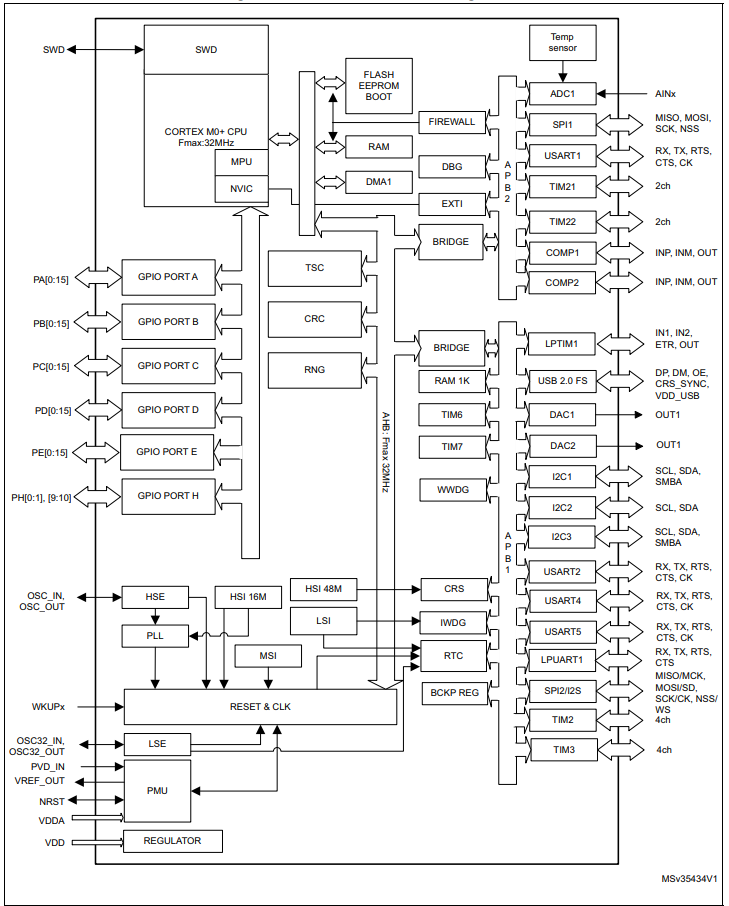
\includegraphics[ width = 0.8\textwidth]{HW_PART/Figs/stm32l072xx.png}
            \caption {Blokový diagram MCU STM32L072xx}
        \end{figure} 
    


\subsubsection{LoRa modul}
      $\text{LoRa}^{\text{TM}}$ je uzavřená technologie, kterou licencuje a vyvíjí firma SemTech. Všechny čipy podporující tuto modulaci nesou označení SX12xx a dělí se na dvě řady.\\
      První řada s čipy SX126x, SX127x, které se liší podle výkonosti nese označení \textit{LoRa Transceivers} je určená pro koncové uzly. Tyto čipy neumožňují multikanálový příjem paketů a jsou omezeny na využití jednoho SF (Spreading Factoru) v danou chvíli.\\
      Naproti tomu druhá řada s čipy SX125x, SX13xx s označením \textit{LoRa Gateways} je mnohem výkonnější a umožňuje automatickou detekci SF přijatého signálu.
      
       \question{Patří to sem???}
       
      Na trhu se nachází nepřeberné množství LoRa modulů, které se liší použitým LoRa čipem, tedy hlavně výstupním výkonem a parametry LoRa modulace a dále komunikačním rozhraním a cenou.\\
      Pro první prototyp měřicí jednotky byl nakonec použit LoRa modul přímo od firmy ST – \textbf{I-NUCLEO-SX1272D} s čipem SX1272, který byl součástí vývojářského kitu a který lze zapojit přímo do Nuclea.
      
      V druhé verzi a plošném spoji byl využit velmi rozšířený modul \textbf{RFM95W} s čipem SX1276, který se těší velké oblíbenosti především díky své nízké cenně.

    \textbf{Specifikace LoRa modulu RFM95W:}
        \begin{itemize}
            \item Celkový vysílací výkon až 161 dB
            \item Programovatelný bitrate až 300 kbps
            \item Citlivost až -148 dBm
            \item Proudový odběr ve SLEEP módu \SI{0.2}{\micro\ampere} 
            \item Proudový odběr ve RX módu kolem \SI{10}{\milli\ampere} 
            \item Proudový odběr ve TX módu \SI{29}{\milli\ampere} při RFOP +13 dBm
        \end{itemize}

     \begin{figure} [!h]
        \centering
        \begin{subfigure}[b]{0.6\textwidth}
             \centering
             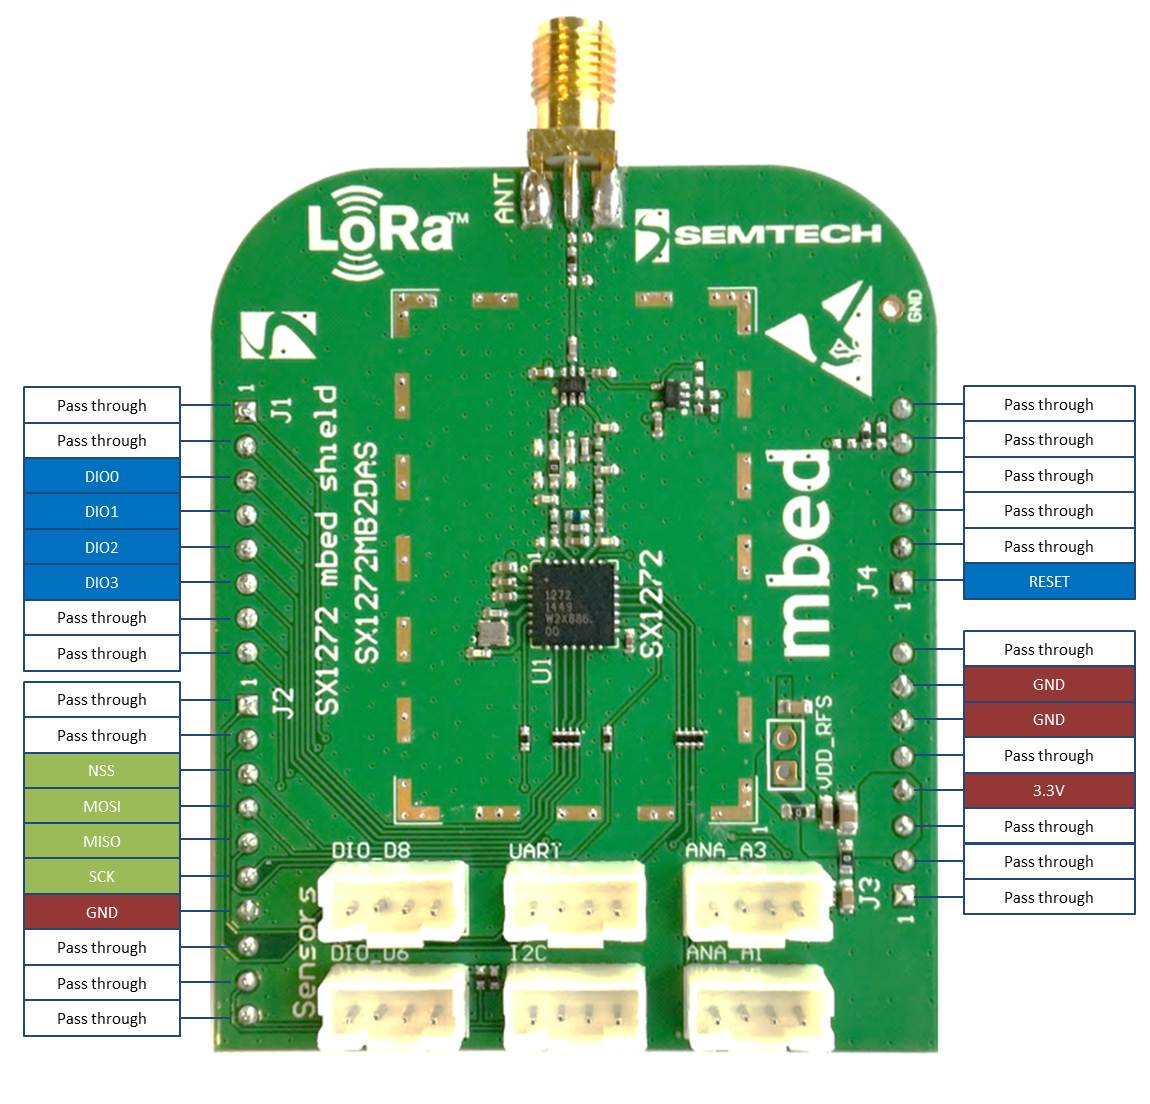
\includegraphics[width=\textwidth]{HW_PART/Figs/SX1272_pinout.jpg}
             \caption {LoRa modul I-NUCLEO-SX1272D}
             \label{fig:y equals x}
         \end{subfigure}
         \hfill
        \begin{subfigure}[b]{0.35\textwidth}
            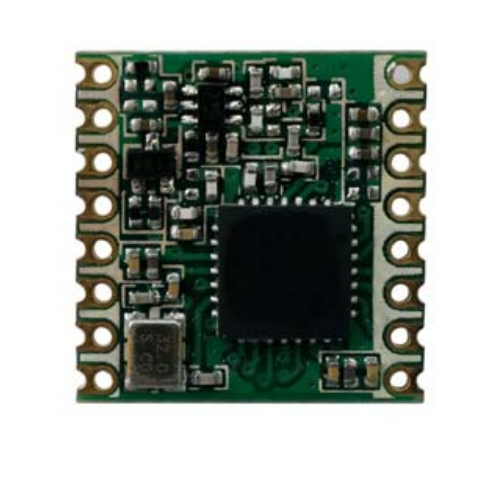
\includegraphics[ width =\textwidth]{HW_PART/Figs/rfm95W.png}
            \caption {LoRa modul RFM95W}
        \end{subfigure}
    \end{figure} 

\subsubsection{Senzor vibrací}
    Výběr akcelerometru byl ovlivněný vhodností pro detekci vibračních signálů a nízkou spotřebou. Tedy postačoval jednoosý akcelerometr s šířkou pásma kolem ... , čemuž vyhovoval akcelerometr \textbf{ADXL1002} od firmy Analog Devices. Tato řada akcelerometrů je přímo určena pro Condition monitoring.\\
    Tyto akcelerometry jsou navíc dodávané na vývojářské destičce  \textbf{EVAL-ADXL1002Z}, která je poměrně tlustá, odolná i vůči silným vibracím, dobře upevnitelná k samotným motorům, a je na ní také umístěn RC filtr, který zamezuje aliasingu.
    Analogový výstup akcelerometru je poté veden koaxiálním kabelem, jehož stínění potlačuje vliv vnějších rušivých polí na přenášený užitečný signál, a je poté zpracováván AD převodníkem na mikrokontroléru. 
    
    \todo{TASK: Refer to place where DSP is explained}
    
    \question{Specifikace koaxiálního kabelu? aktivní stínění?}
    
    \question{Jaký je běžný rozsah frekvenčních signálů a stačí jednoosý??, co je noise floor?}
    \question{Na co tam je RC filter vlastne - aliasing/sum?}

    \answer{rozsah, noise floor u analogového/ rozlišení u digitálního, šířka pásma/vzorkovací frekvence}

    \textbf{Specifikace akcelerometru ADXL1002:}
        \begin{itemize}
            \item Jednoosý akcelerometr typu MEMS (mikroelektromechanický)
            \item Šířka pásma $11 kHz$
            \item Měřicí rozsah $\pm50 g$
            \item Citlivost $40 mV/g$, při nulovém $g$ je na výstupu polovina napájecího napětí
            \item Analogový výstup
            \item Proudový odběr v měřícím módu \SI{1}{\milli\ampere}
            \item Proudový odběr v STDBY módu  \SI{225}{\micro\ampere} 
        \end{itemize}
        
    \begin{figure} [!hbp]
        \centering
        \begin{subfigure}[b]{0.6\textwidth}
             \centering
             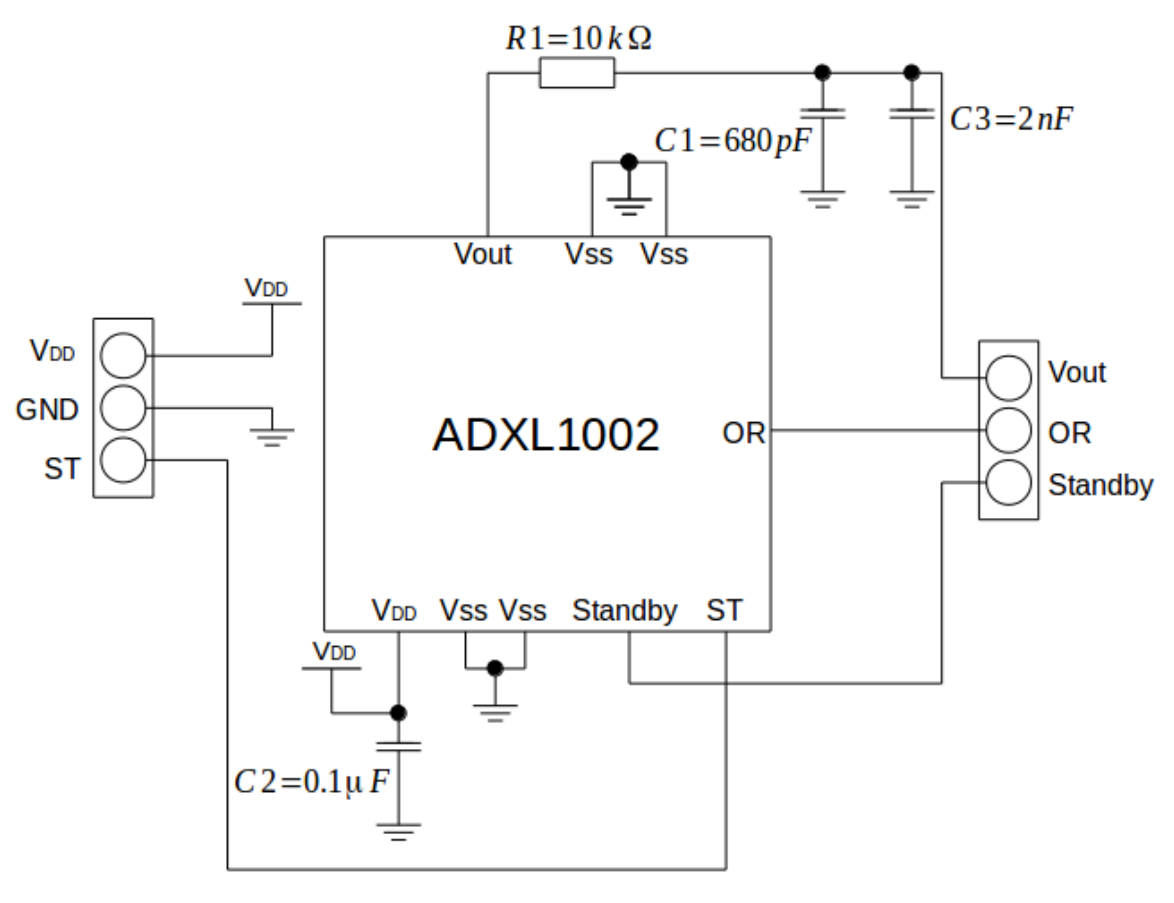
\includegraphics[width=\textwidth]{HW_PART/Figs/adxl1002.png}
             \caption {Schéma vývojové desky EVAL-ADXL1002Z}
             \label{fig:y equals x}
         \end{subfigure}
         \hfill
        \begin{subfigure}[b]{0.6\textwidth}
            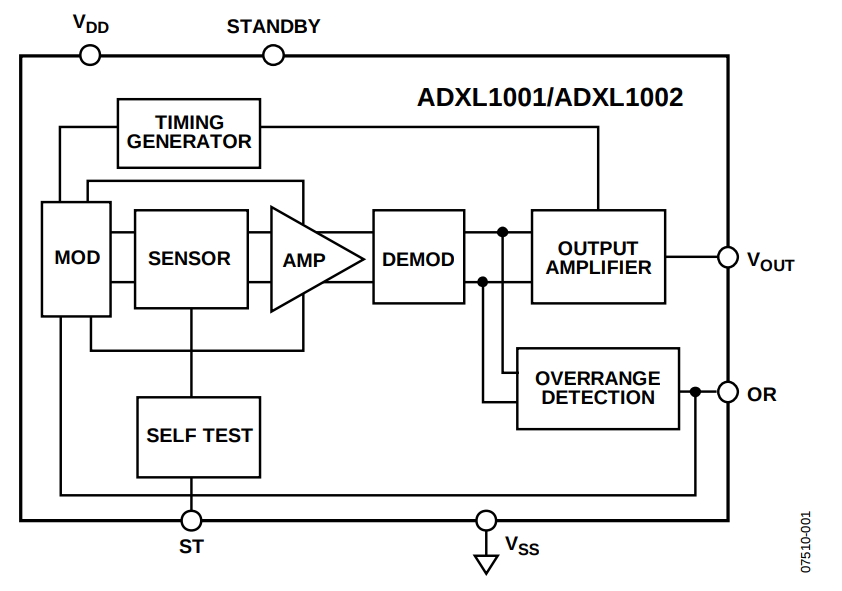
\includegraphics[ width =\textwidth]{HW_PART/Figs/adxl1002_functionaldiagram.png}
            \caption {Blokový diagram ADXL1002}
        \end{subfigure}
    \end{figure} 
    
    


\subsubsection{Teplotní senzor}
    Pro monitorování teploty bylo vybráno digitální teplotní čidlo \textbf{TMP75} od firmy Texas Instruments, které pro měření využívá 12bitový převodník. Jedná se o poměrně rozšířený senzor komunikující po I2C sběrnici, který je díky své malé spotřebě vhodný zejména do zařízení, které jsou poháněny baterií.

    \textbf{Specifikace teplotního čidla TMP75:}
        \begin{itemize}
            \item Přesnost $\pm$ \ang{1}C
            \item Programovatelné rozlišení 9-12 bitů
            \item Rozsah \ang{-40}C-\ang{+125}C
            \item Proudový odběr \SI{50}{\micro\ampere}
        \end{itemize}
     
     \begin{figure} [!hbp]
        \centering
        \begin{subfigure}[!h]{0.5\textwidth}
             \centering
             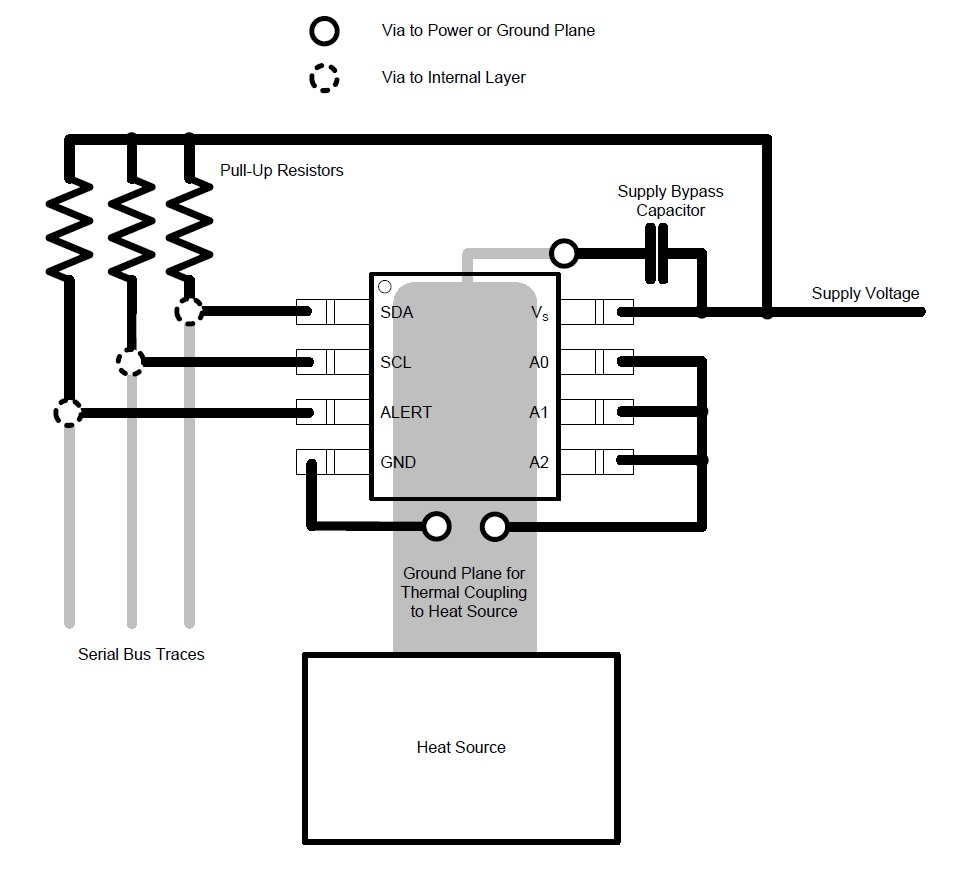
\includegraphics[width=\textwidth]{HW_PART/Figs/tmp75_connection.jpg}
             \caption {Schéma připojení TMP75}
         \end{subfigure}
         \hfill
        \begin{subfigure}[!h]{0.45\textwidth}
            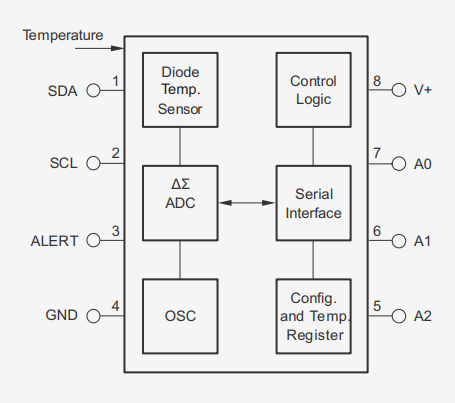
\includegraphics[ width =\textwidth]{HW_PART/Figs/tmp75_functionaldiagram.png}
            \caption {Blokový diagram TMP75}
        \end{subfigure}
    \end{figure} 

\subsection{Celkový design} 

\subsubsection{První prototyp}
    První verze měřicí jednotky byl vytvořen pomocí vývojářského kitu NUCLEO s procesorem STM32L073RZ, LoRa modulem s čipem SX1272 a nepájivým polem, do kterého byly připojeny vývody senzorů. Oba dva byly napájeny z Nuclea a byly k nim přidány kondenzátory pro blokování napájení. Výsledné zapojení lze vidět na obrázku.
    
    \todo{IMAGE: Make photo}
    
\subsection{Druhá verze}
    Druhá verze měřící jednotky byla vytvořena bez Nuclea zapájením čipu STM3272KZ na adaptor a připojením LoRa modulu RFM95W a senzorů na univerzální destičce...
    














\section{Řídicí jednotka (LoRa Gateway)}
\subsection{Výběr komponent}
\subsubsection{Mikrokontrolér (MCU)}

    Vlastní LoRa brána může být postavena spíše minimalisticky za použití určitého mikrokontroléru, tedy se slabým výkonem, ale nízkou cenou a spotřebou – například jako další STM32 jednotka s Ethernet nebo WiFi modulem nebo pomocí oblíbeného vývojářského čipu ESP8266/ESP32. Opačný přístup by bylo postavení brány s výpočetně silnějším počítačem a operačním systémem, tedy s velkým výkonem, ale vyšší cenou a spotřebou.
    Pro realizaci brány bylo ale nakonec použité \textbf{Raspberry Pi} verze 3 model B. 
    Motivací výběru Raspberry po zvážení kritérií popsaných výše byl zejména dostatečný výpočetní výkon, vývojářská podpora a výhody operačního systému. Spotřeba brány není tak důležité kritérium jako u koncových zařízení, protože brána může mít stálý zdroj napájení. Raspberry byl tedy jakýsi kompromis mezi výkonem a cennou.

\textbf{Specifikace Raspberry Pi model B:}
    \begin{itemize}
        \item 64 bitový čtyřjádrový procesor Broadcom BCM2837 1.2GHz, 1 GB RAM
        \item 40 externích GPIO pinů
        \item BCM43438 WLAN a Bluetooth Low Energy (BLE)
        \item 4 USB porty, HDMI, 3.5 mm jack
        \item Micro SD port
    \end{itemize}
    
\subsubsection{LoRa modul}
    Z důvodů popsaných v ... byla brána navržená jako jednokanálová. Pro LoRa komunikaci tedy nebylo nutné používat čipy ze série SX125x, SX13xx, a byl proto v obou verzích využit stejný čip jako u měřicí jednotky - SX1272 v první verzi a RFM95W ve druhé verzi.
    
\subsubsection{Displej}
    
 \subsubsection{První prototyp}
    První verze brány byla vytvořena pouze s LoRa modulem určeným původně pro Nucleo I-NUCLEO-SX1272D, který musel být s GPIO piny propojen jednotlivými drátky.
    
    \todo{IMAGE: Make picture of GW.}

 \subsubsection{Konečná verze}
 
 
 
 \question{TYPOGRAFIE - jednoty kurzivou nebo ne?}

\question{TYPOGRAFIE - pomlcky vs spojovniky}

\question{TYPOGRAFIE - stupen - mezera nebo ne}

\question{TYPOGRAFIE - mezery za jednotkami}


\part{SW Design}

%!TEX ROOT=ctutest.tex

%% Na obrazku lze videt xx obrazek ukazuje
%% trpny rod

\chapter{Softwarová implementace}

\section{Celkové chování systému}

\subsection{Komunikační protokol}
    Pro účely aplikace byl navržen komunikační protokol sloužící k rozlišení funkcionality jednotlivých paketů, přehlednou práci s přijatými nebo odesílanými daty a hlavně velmi dobrou budoucí rozšířitelnost celého systému.\\
    Každý radiopaket má pevně danou dvoubajtovou hlavičku, jež obsahuje  parametr \textit{CMD} determinující význam paketu a parametr \textit{sessionId}, který si lze představit podobně jako IP adresu, tedy specifikuje, komu je paket určen.\\
    Komunikační protokol je specifikovaný na straně brány v souboru \textit{radio\_packet.py} a na straně uzlu \textit{radio\_protocol.h}. 
    
    \todo{IMAGE: Doplnit obrázky}
    

\subsection{Zahájení komunikace – Join Process}
    Každá měřicí jednotka musí po svém restartu nejdříve zažádat o autorizaci u nejbližší brány. Tento proces probíhá prostřednictvím radiopaketu – JoinRequest, který je opakovaně odesílán, dokud brána neodpoví. Obsahem paketu je zejména unikátní čtyřbajtový identifikátor procesoru – \textit{uniqueId}, nulová jednobajtová adresa – \textit{sessionId} a časová známka sloužící pro pozdější časovou synchronizaci.\\
    Jakmile brána tento paket přijme je podle unikátní adresy zpracován a na jednotku je zpětně odeslán radiopaket JoinResponse s načtenou konfigurací z databáze a již konkrétní sessionId, která se dále využívá v průběhu celé další komunikace.
    
 \todo{TASK: Doplnit obrázky}
 
 \subsection{Nahrání konfigurace}
 \subsection{Konfigurace}


\section{Měřící jednotka (LoRa Node)}
\subsection{Použité softwarové nástroje}

%% opravdu to sem patri
    Software měřící jednotky byl napsán v programovacím jazyce C za použití vývojového prostředí Atollic TrueSTUDIO.\\
    Projekt byl založený na balíku dodaném firmou ST pro vývoj aplikací využívající LoRu – \textit{I-CUBE-LRWAN Expansion Package}.\\ 
    Z tohoto balíku byly využity zejména moduly pro obsluhu RF LoRa čipů od firmy Semtech SX1272/SX1276 (tedy PHY vrstva LoRaWAN protokolu), inicializace některých periferií a dodatečné nástroje jako třeba logování na konzoli.
    Implementace MAC vrstvy LoRaWAN protokolu využita nebyla z důvodů popsaných...
    \begin{figure} [h]
	    \centering
	    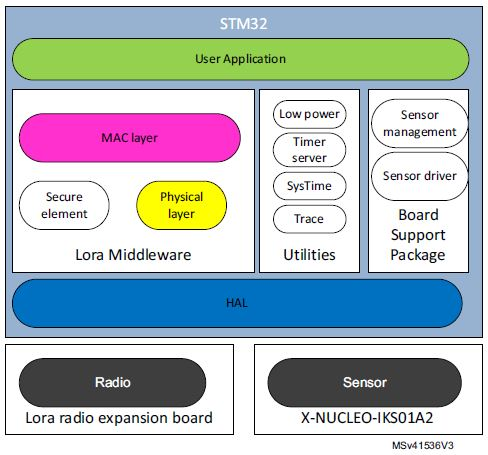
\includegraphics[ width = 0.8\textwidth]{SW_PART/Figs/st_loraextension.jpg}
        \caption {Hierarchie SW nástrojů dodaných firmou ST}
    \end{figure}  
    
    \todo{Misto, kde zduvodnim, proc nepouzivam LoRaWAN}
    
\subsection{Měřící jednotka – STATUS mód}
\subsection{Měřící jednotka – DEBUG mód}

   
%%Softwarový vývoj postavený na platformě ST může probíhat několika odlišnými způsoby. Lze využívat knihovnu obsahující pouze registry procesoru – CMSIS, kterou dodává samotný ARM nebo nízkoúrovňové knihovny LL (Low Level) či již komplexní knihovny HAL (Hardware Abstraction Layer), jejichž dodavatelem je ST. Pro vývoj měřící jednotky byl pou nakonec použita kombinace p  Obsluha komunikace MCU přes UART byla například naprogramována pouze pomocí CMSIS, obsluha AD převodníku pomocí LL a obsluha I2C pomocí HAL.
 %%
 
\section{Řídicí jednotka (LoRa Gateway)}
\subsection{Použité softwarové nástroje}
    Na Raspberry Pi byl v první řadě nainstalován operační systém Raspbian \cite{cite:3} ve verzi bez uživatelského rozhraní, který je založený na linuxovém Debianu a optimalizovaný pro Raspberry Pi. Pro samotný software řídící jednotky byl poté využit skriptovací programovací jazyk Python. Ten díky široké škále knihoven, které lze do projektu snadno importovat, usnadňuje vývojáři práci.\\
    Pro obsluhu GPIO pinů a periferií Raspberry jako SPI a UART byla využita knihovna \textit{wiringpi}.
    HTTP komunikaci s Node-RED serverem zabezpečovala knihovna \textit{requests} a TCP/IP komunikaci s TTN serverem knihovna \textit{socket}.
  
\subsection{Struktura aplikace – vícevláknový přístup}
    Z hlediska logické struktury byla aplikace rozdělena na hlavní vlákno a jednotlivá vlákna reprezentující připojené měřicí jednotky.\\
    Úkolem hlavního vlákna je neustále obsluhovat LoRa modul - přijímat a odesílat pakety. Tato obsluha musí probíhat neustále a nesmí být závislá na jiných okolnostech zdržujících její průběh, jako je komunikace s Node-RED servrem či zpracovávání přijatých informací.\\
    Ostatní vlákna zabezpečují úkoly jednotlivých měřicích jednotek. Zpracovávají přijatá naměřená data – radiopakety StatusInfo a odesílají je spolu s dalšími informacemi do Node-RED serveru.
   
    \todo{TASK:Vizualization of multithreading access}
    
    


\subsection{Řízení přístupu k rádiovému rozhraní}
    Jelikož řídicí jednotka umožňuje komunikovat s více měřicími jednotkami současně, je třeba brát ohled na využití rádiového LoRa modulu.\\
    V jednu chvíli se totiž může stát, že jedna jednotka bude odesílat informace o měření – radiopaket StatusInfo a druhé bude třeba z brány odeslat konfiguraci.
    
    Zprávy ze všech měřicích jednotek jsou přijaty v hlavním vlákně a to s nimi nakládá podle modelu producent-konzument. Přijatý paket rozešle do vláken všech komunikujících jednotek, které pak paket zpracují podle toho, jestli odpovídá jeho parametr \textit{sessionId}.\\
    Zprávy, které potřebuje brána odeslat daným měřicím jednotkám jsou nejprve vytvořeny v příslušném vláknu a přes společnou odesílací frontu jsou sdíleny s hlavním vláknem.
    
    Pro bránu je prioritní downlik, tedy odesílání zpráv. V hlavním cyklu se vždy kontroluje podmínka, že odesílací fronta je prázdná, pokud je přechází brána do RX (přijímacího) módu, ve kterém setrvá do vypršení timeoutu. Jakmile se tak stane a v odesílací frontě se objeví paket, je okamžitě odeslán a pokračuje se v cyklu. 
    \begin{figure} [h]
	    \centering
	    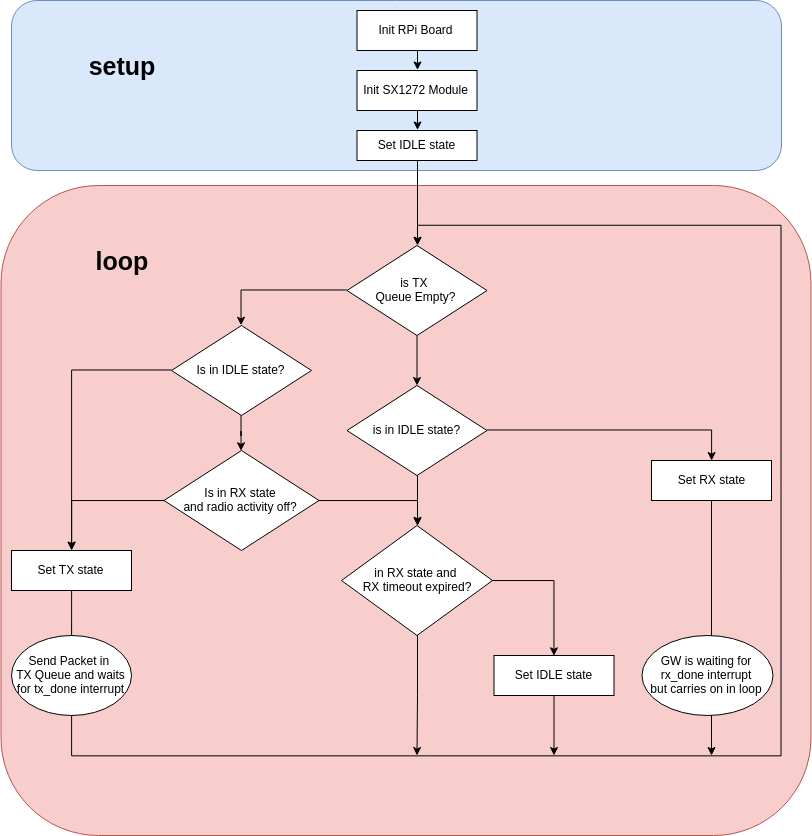
\includegraphics[ width = 0.9\textwidth]{SW_PART/Figs/GW_loop.png}
        \caption {Základní řídící smyčka hlavního vlákna brány}
    \end{figure}  
    
    
   
   
   
\section{Aplikační IoT server a databáze}
    Aplikační server a databáze jsou logicky odděleny od řídicí jednotky na Raspberry a mohou být umístěny kdekoliv na internetu, což umožňuje větší modularitu celého systému. Ve vytvořené demo aplikace byly ale všechny části umístěny na Rapberry Pi. Data jsou z řídicí jednotky nejprve umístěna do databáze. K vizualizaci slouží jednoduché uživatelské rozhraní, které data získává opětovnými SQL dotazy na databázi.
    
\subsection{Použité softwarové nástroje}
    Logika aplikačního serveru byla vytvořena na platformě Node-RED. Tento nástroj, vyvíjený společností IBM, je postavený na javascriptovém serveru Node.js a uživateli umožňuje pohodlně propojovat hardwarová zařízení, APIs (aplikační rozhraní) a online služby za pomocí flowchartového programování a to vše ve webovém rozhraní.\\ 
    Pro ukládání dat byla využita opensourcová databáze PostgreSQL. Jedná se o relační databázi, kde jednotlivé klíče (unikátní identifikátory typu GUID) udávají vztahy mezi tabulkami a záznamy v databázi.


\subsection{Komunikace s řídící jednotkou}
    Řídicí jednotka komunikuje se serverem prostřednictvím HTTP požadavků.\\
    Konfiguraci a informace o konkrétních uzlech získává brána prostřednictvím dotazu HTTP GET na url:\\ 
    \texttt{http://<Node-RED ip>:1880/app/config} či \\
    \texttt{http://<Node-RED ip>:1880/app/node\_params},\\
    kde v hlavičce dotazu specifikuje identifikační číslo daného uzlu. Jako odpověď přichází záznamy z databáze ve formátu JSON. IP adresa serveru se liší podle toho, kde je server umístěn, port je standardní – 1880.\\
    Pokud měřící jednotka pracuje ve STATUS módu, jsou do aplikačního serveru posílána data z měření, čehož lze docílit dvěma různými způsoby. Data lze odesílat na aplikační vrstvě osi-iso modelu pomocí HTTP POST dotazu na url:\\
    \texttt{http://<Node-RED ip>:1880/app/statusinfo}, \\
    kde se data společně s identifikačním číslem uzlu nacházejí v těle dotazu, nebo prostřednictvím transportní vrstvy pomocí UDP paketů na speciální port 8888.
    
    \todo{TASK: Vlozit tabulku s popisem url}
    
\subsection{Komunikace s aplikacemi třetích stran – REST API}
    Krom řídící jednotky je server připraven poskytovat data i aplikacím třetích stran, k čemuž slouží rozhraní vybudované na základě REST-JSON. S tímto rozhraním pak může komunikovat jakákoli další klientská aplikace, tedy například webový interface, který data získává pomocí javascriptu, nebo další připojený systém, což umožňuje koncovému uživateli velikou flexibilitu a rozšiřuje možnosti využití systému. 
    Data lze získat přes HTTP GET dotaz na stejné url jako v případě vkládání dat a pro přesnější výsledky je v rozhraní systému umožněno SQL-like dotazování použitím základních SQL struktur.
    
    \todo{TASK: Doplnit SQL-like dotazovaní}
  
    \todo{IMAGE: Doplnit o obrázek ze serveru}  
   
\subsection{Datový model}
    Pro účely aplikace byl vytvořen datový model, postavený na principech modelu relační databáze, který je znázorněn na obrázku.
    \begin{figure} [!h]
	    \centering
	    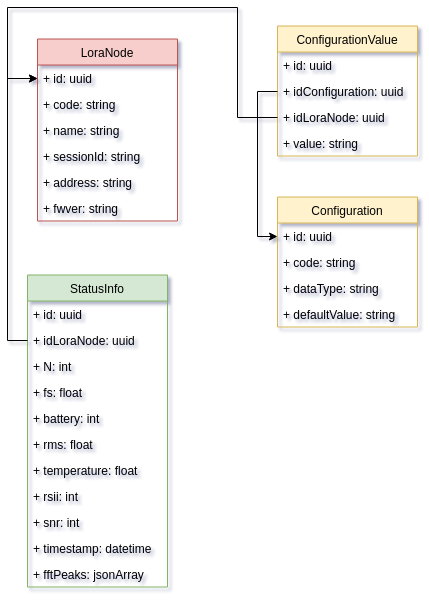
\includegraphics[ width = 0.8\textwidth]{SW_PART/Figs/data_model.png}
        \caption {UML diagram datového modelu aplikace}
    \end{figure} 
    
\subsection{Uživatelské rozhraní}
    V rámci serveru bylo vytvořeno také jednoduché uživatelské rozhraní, ve kterém jsou znázorněny časové změny monitorovaných veličin (teploty, RMS, stavu baterie, krest faktoru), nejvýznamnější píky ve frekvenčním spektru vibračního signálu a dodatečné informace o RSSI, SNR a časové známce   posledního přijatého paketu. Celé uživatelské rozhraní bylo vytvořeno za pomocí doplňku \textit{node-red-dashboard}.
    
    \todo{IMAGE: Pekny obrazek uzivatelskeho rozhrani}
    

    
    




%\blindmathtrue

%\blinddocument


\appendix

\printindex

\appendix

\bibliographystyle{amsalpha}
\bibliography{ctutest}

%\ctutemplate{specification.as.chapter}

\end{document}